\section{\acl{dw}} \label{sec:dw}

Ein \acf{dw} ist \glqq eine fachlich orientierte, integrierte, nicht volatile und in der Zeit veränderliche Sammlung von Daten zur Unterstützung von Entscheidungen\grqq{} \cite{dworiginal}. Die Eigenschaft der Fachorientierung eines \ac{dw} ermöglicht auch die Nutzung solcher Systeme für Forschungszwecke \cite{dwhcliniinv}. Ein \ac{dw} ist auch \glqq eine physische Datenbank, die eine integrierte Sicht auf beliebige Daten zu Analysezwecken ermöglicht\grqq{} \cite{dwgoeken}. Die folgenden Eigenschaften lassen sich aus der Definition ableiten \cite{planungdatawarehouse}.

\begin{itemize}
	\item Fachorientierung: Die Datenstruktur im \ac{dw} wird für die Unterstützung von klinischen Problemstellungen und Entscheidungen optimiert und somit für die Berechnung von Kennzahlen und deren Zuordnung
	\item Integration: Daten aus diversen Datenquellen werden in getrennte \acp{db} integriert, z. B. die Informationen der verschiedenen Quellsysteme in einem Krankenhaus werden in unterschiedlichen \acp{db} des Staging Bereichs eines \ac{dw} gesammelt
	\item Beständigkeit: Die geladenen Daten im \ac{dw} bleiben unverändert
	\item Historisierung: Die über lange Zeit gespeicherten Daten ermöglichen die Erkennung von Entwicklungen und Trends in den Daten
\end{itemize}

Die Anwendungsbereiche von \acp{dw} in klinischen Einrichtungen umfasst die Bereitstellung von Informationen, komplexe und flexible Datenanalyse, die Entwicklung von Forschungsprojekten und die Unterstützung der Planungsprozesse \cite{planungdatawarehouse}.

Die Architektur eines \ac{dw} besteht aus fünf Ebenen \cite{dwbauer}. Die Ebene der Datenquellen umfasst die internen und externen Datenquellen mit relevanten Daten \cite{dwgoeken}. In der Datenerfassungsebene werden diese Daten mit Hilfe von \ac{etl}-Prozessen (\ref{subsec:etl}) für das Laden in das zentrale \ac{db}-System (Datenhaltungsebene) extrahiert, aufbereitet und konvertiert \cite{dworiginal}. Diese zentrale \ac{db} ist in mehreren \acp{db} aufgeteilt, und jede davon stellt eine bestimmte Datenquelle dar \cite{dwgoeken}. In der Datenbereitstellungsebene werden die gespeicherten Daten für multidimensionale Analysen aufbereitet \cite{dwbauer}. Auf der Präsentationsebene befinden sich Anwendungsprogramme mit Zugriff auf die aufbereiteten Daten für die Analyse \cite{dwtool}.

\subsection{\acs{etl}} \label{subsec:etl} 

Die \acf{etl}-Prozesse oder Erfassungsprozesse in einem \ac{dw} dienen der Aufbereitung und dem Laden der Daten in die \acp{db} des \ac{dw}. Diese Prozesse sind je nach Datenmenge und Design des \ac{dw} sehr zeitintensiv \cite{dwbauer, dwtool}.

Zuerst werden bei der Datenextraktion die Daten aus den verschiedenen Datenquellen extrahiert und in einen Zwischenspeicher übertragen, dem sogenannten Staging Bereich \cite{dwtool}. In diesem Prozess werden die ersten Umwandlungen, wie die Pseudonymisierung von personenbezogenen Daten und die Konvertierung von Datentypen zwischen dem Quellsystem und dem \ac{dw}, vorgenommen \cite{dwbauer}.

Nach der Datenextraktion werden die Daten transformiert. Ziel der Transformation ist eine hohe Qualität der Daten zu gewährleisten. Damit werden die extrahierten Daten bereinigt, harmonisiert und zusammengeführt. Bei der Transformation werden Fehler und Inkonsistenzen beseitigt. Ein weiterer Aspekt der Datentransformation ist die Erstellung von Metadaten und künstlichen Schlüsseln zur Erleichterung der Referenzen auf die Datensätze im \ac{dw}, denn in manchen Fällen werden die Schlüssel der Quellsysteme nicht verwendet, denn zwei oder mehrere Quellsystemen können dasselbe Schlüsselschema haben \cite{dwbauer, dwtool}, z. B. die Nutzung von fortlaufenden Nummern als Primärschlüssel für die Identifikation von Diagnosen in verschiedenen Datenquellen.

Die Ladephase ist die Letzte im \ac{etl}-Prozess. Damit werden die transformierten Daten physikalisch in die Zieltabellen des \ac{dw} überführt \cite{dwgoeken, dwtool}.

Ein Beispiel eines \ac{etl}-Prozesses ist in der \ref{fig:dizummz} im Kapitel \glqq Realisierung\grqq{} (\ref{ch:results}) dieses Projekts dargestellt.

\subsection{Datenmodell eines \acs{dw}} \label{subsec:datamodel}

Das Datenmodell eines \ac{dw} orientiert sich an Sachverhalten eines Unternehmens, und somit ist ein \ac{dw} themenorientiert und bietet eine aggregierte Sicht auf das Geschehen \cite{dwgoeken}.

Das Datenmodell eines \ac{dw} ist multidimensional und somit weit verbreitet für die Darstellung analytischer Daten, außerdem ist dieses Modell relativ einfach und vereinfacht die Modellierung der physikalischen \ac{db} eines \ac{dw} \cite{dwbauer}. Andere Vorteile dieser Modellierungsart sind die Performanz und die verständliche Darstellung der Daten für wissenschaftliche Fragestellungen \cite{dwtool}.

Das multidimensionale Modell besteht aus Dimensionen und Fakten \cite{dworiginal}. Die Dimensionen (Dimensionstabellen) sind Konzepte oder Hierarchien, um die Daten zu kategorisieren. Die Fakten (Faktentabellen) sind Beobachtungen, Berechnungen oder Messungen \cite{dwtool}. Der Hauptschlüssel der Faktentabellen ist meist ein künstlicher Schlüssel, der die Kombination der Hauptschlüssel der Dimensionstabellen enthält \cite{dwbauer, dwtool}. 

Die Daten in einem multidimensionalen Datenmodell werden in einer physikalischen \ac{db} eines \ac{rdms}, wie PostgreSQL oder Microsoft SQL Server, meist in einem Sternschema gespeichert und dargestellt \cite{dworiginal}. Seinen Namen verdankt das Schema seiner Ähnlichkeit mit einem Stern, wie in der \ref{fig:starschema} dargestellt wird \cite{dwtool}.

\clearpage

\begin{figure}[ht]
	\centering
	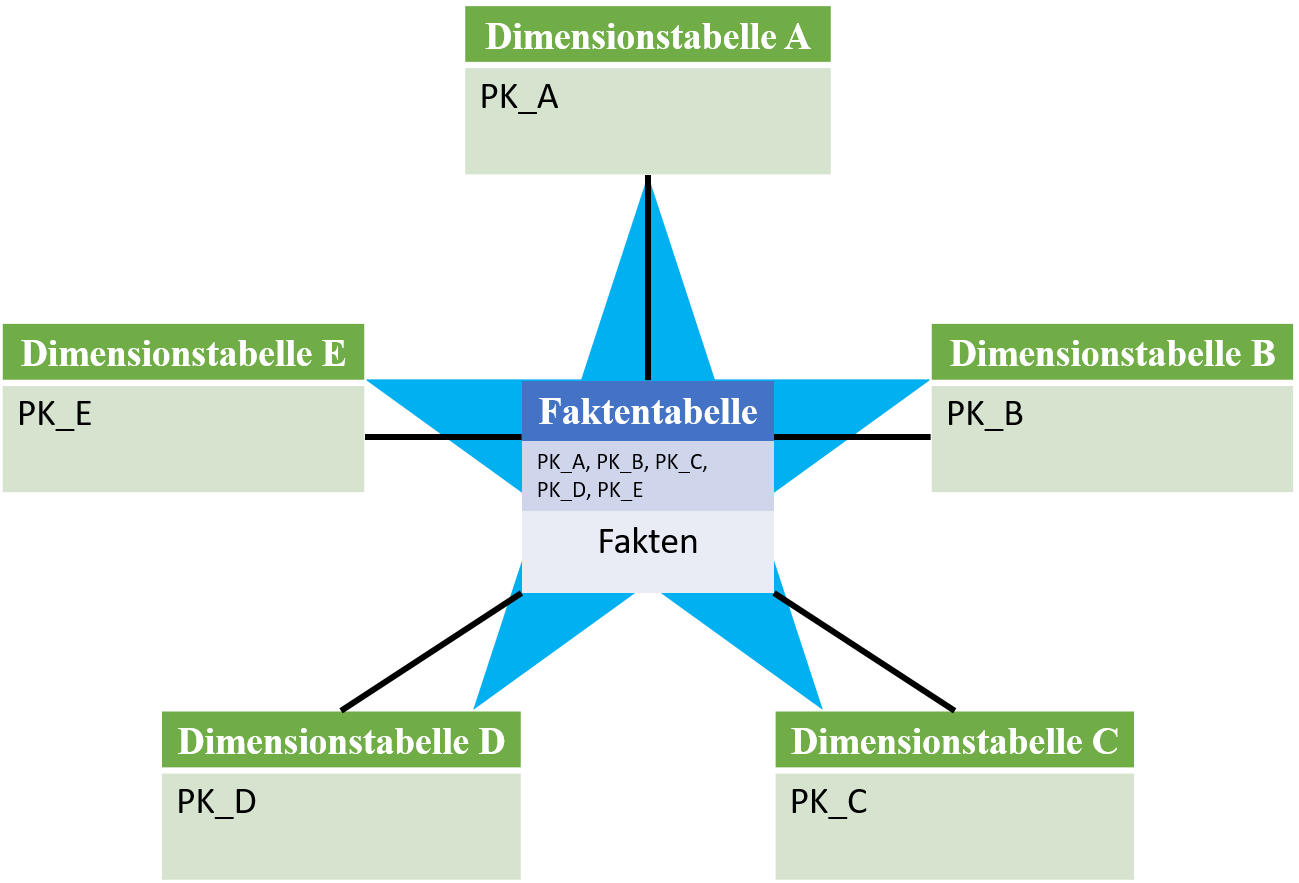
\includegraphics[height=8.5cm]{figures/starschema}
	\caption[Sternschema]{Sternschema. Die Dimensionstabellen beinhalten Kategorien. Die Faktentabelle beinhaltet die Hauptschlüssel der Dimensionstabellen und die Ergebnisse von Analysen. \glqq PK\_\grqq{} stellt die Hauptschlüssel der Tabellen dar.}
	\label{fig:starschema}
\end{figure}
